\subsection{Factorisation ILU(k) avec renumérotation des cellules}
Lorsque nous renumérotons les cellules, nous obtenons un graphe de tâches différent.
%
Une numérotation rouge-noir donne un graphe très large avec seulement 2 niveaux de hauteur.
%
Nous pouvons aussi utiliser une numérotation de type {\em nested dissection} pour obtenir un autre type de graphe.
%
Ce graphe aura la forme d'un arbre.
%
De plus, augmenter le niveau de remplissage de l'algorithme ILU(k) créera de nouvelles connexions dans le graphe.
%
Nous allons donc utiliser notre simulateur avec une numérotation nested dissection des matrices.
%
Nous définissons les paramètres 0,6 pour les effets caches et 2 pour le coût d'ordonnancement.
%
Donc le temps d'exécution d'une tâche est 2 fois moins long que le temps d'ordonnancement.
%
En regardant le graphe de tâches (Fig.~\ref{fig:ilu_ordering_F}), on s'aperçoit que le graphe est plus large que haut.
%
L'opérateur F devrait donnait de très bons résultats sur ce graphe.
%
Mais comme les effets cache sont importants, il est possible que l'opérateur D puisse faire aussi bien.
%
Lorsque nous regardons les résultats (Table.~\ref{tab:ilu0_nested_0.6_2}), l'opérateur F donne les meilleurs résultats.
%
En créant plus de tâches que de coeurs de calcul par niveau, on autorise un meilleur équilibrage de charge pour les niveaux qui n'ont pas assez de tâches.
%
L'opérateur C n'est pas du tout efficace car le graphe n'est pas assez haut.


%   (-_-)   %
\begin{center}
  \begin{tabular}{|c|c|c|c|c|c|c|c|c|c|c|}
    \hline
    \multicolumn{11}{|c|}{Types d'agrégations}\\
    \O & D(16) & D(64) & D(256) & D(1500) & D(2048) & F(24) & F(36) & F(42) & F(64) & C \\
    \hline
    250005 & 83549 & 72145 & 67706 & 65790 & 66162 & 65070 & 61493 & 61195 & 61219 & 246386 \\
    \hline
  \end{tabular}
  \captionof{table}{Résultats du simulateur d'exécution de tâches avec une granularité très fine sur 12 coeurs de calculs.}
  \label{tab:ilu0_nested_0.6_2}
\end{center}


%   (-_-)   %
\begin{figure}[t!]
  \centering
  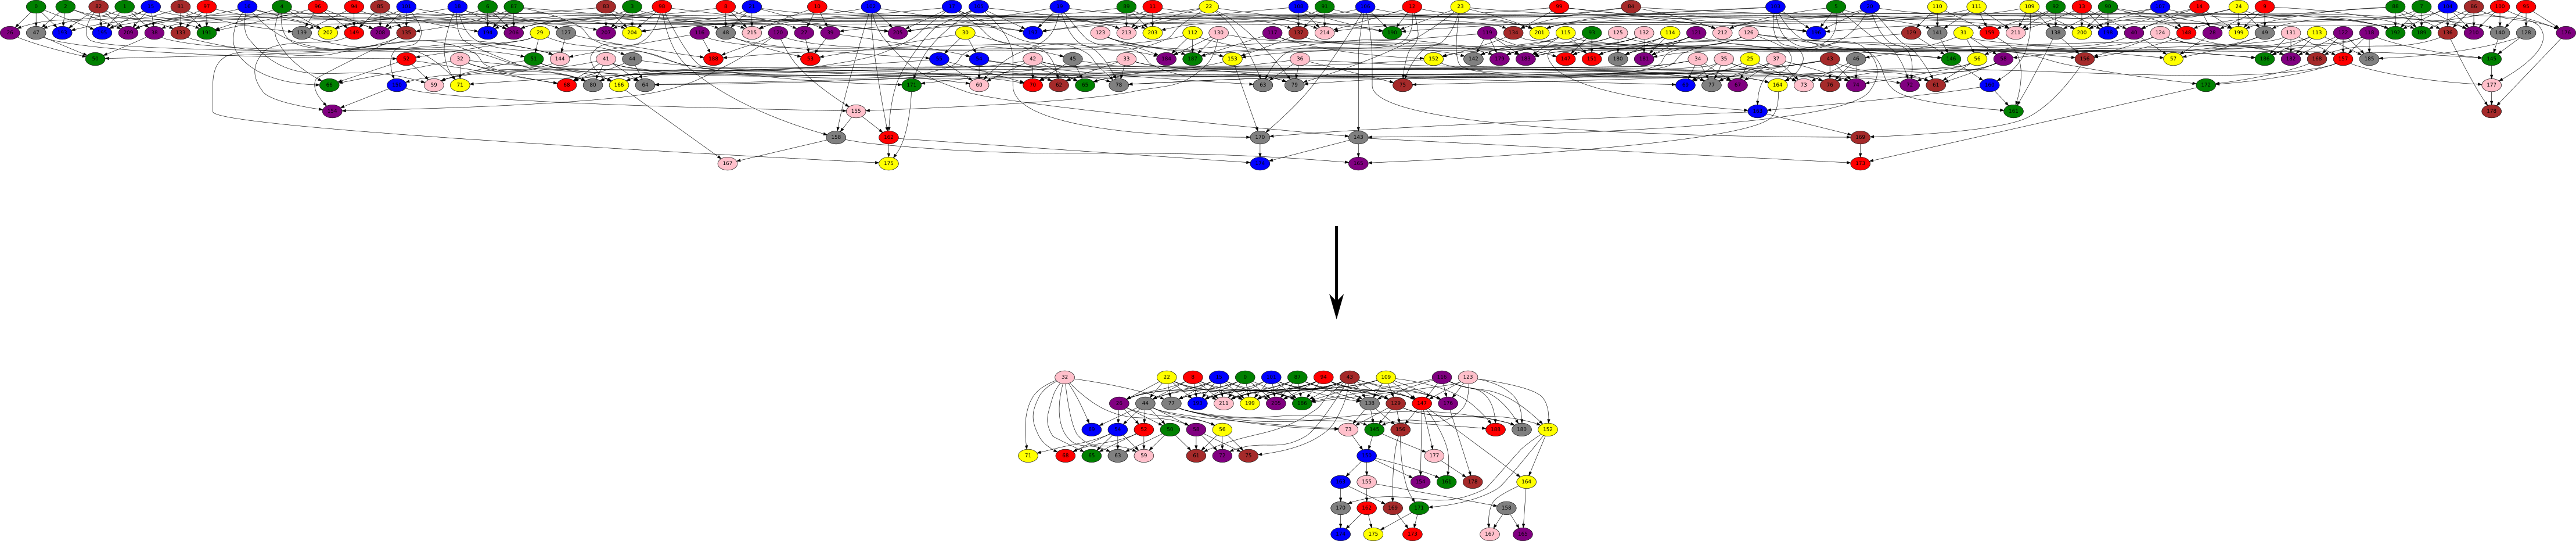
\includegraphics[width=\textwidth]{ilu_ordering_F}
  \caption{Exemple de graphe avec un ordering nested dissection. Nous avons appliqué l'opérateur F.}
  \label{fig:ilu_ordering_F}
\end{figure}


Supposons dans un deuxième temps que les tâches soient plus grosses et que le paramètre cache soit moins important.
%
Nous travaillerons donc avec les valeurs 0,8 pour les effets caches et 0,5 pour le coût d'ordonnancement.
%
Ordonnancer une tâche ne coûte plus que la moitié du temps de l'exécution de la tâche.
%
Tout comme l'exemple précédent, l'opérateur F donne les meilleurs résultats.
%
Le graphe n'est pas assez haut pour pouvoir obtenir de bons résultats avec les autres opérateurs.


%   (-_-)   %
\begin{center}
  \begin{tabular}{|c|c|c|c|c|c|c|c|c|c|c|}
    \hline
    \multicolumn{11}{|c|}{Types d'agrégations}\\
    \O & D(16) & D(64) & D(256) & D(1500) & D(2048) & F(24) & F(36) & F(42) & F(64) & C \\
    \hline
    125002 & 80849 & 77157 & 75604 & 75602 & 76250 & 73319 & 72616 & 72433 & 72251 & 123946 \\
    \hline
  \end{tabular}
  \captionof{table}{Résultats du simulateur d'exécution de tâches avec une granularité grossière sur 12 coeurs de calculs.}
  \label{tab:ilu0_nested_0.8_0.5}
\end{center}


Nous allons maintenant augmenter le niveau de remplissage de l'algorithme ILU.
%
Un remplissage de niveau 2 permet d'augmenter le nombre d'arêtes dans le graphe est de le rendre plus haut (Fig.~\ref{fig:ilu_ordering2_F}).
%
Le nombre de tâches par niveau dans le graphe n'est pas uniforme.
%
Nous allons donc réessayer les différents d'opérateurs d'agrégation sur ce nouveau graphe.
%
Nous réutilisons les paramètres du simulateur cité plus haut (0,6 pour les effets cache et 2 pour l'ordonnancement).
%
Les résultats de la table~\ref{tab:ilu2_nested_0.6_2} nous montrent que l'opérateur F est toujours le plus efficace.
%
Par contre, la différence avec l'opérateur D est réduite.


%   (-_-)   %
\begin{center}
  \begin{tabular}{|c|c|c|c|c|c|c|c|c|c|c|}
    \hline
    \multicolumn{11}{|c|}{Types d'agrégations}\\
    \O & D(16) & D(64) & D(256) & D(1500) & D(2048) & F(24) & F(36) & F(42) & F(64) & C \\
    \hline
    250008 & 85977 & 74584 & 69348 & 69398 & 69118 & 68156 & 67863 & 67977 & 68387 & 224098 \\
    \hline
  \end{tabular}
  \captionof{table}{Résultats du simulateur d'exécution de tâches  avec ILU(2) et une granularité très fine sur 12 coeurs de calculs.}
  \label{tab:ilu2_nested_0.6_2}
\end{center}


%   (-_-)   %
\begin{figure}[t!]
  \centering
  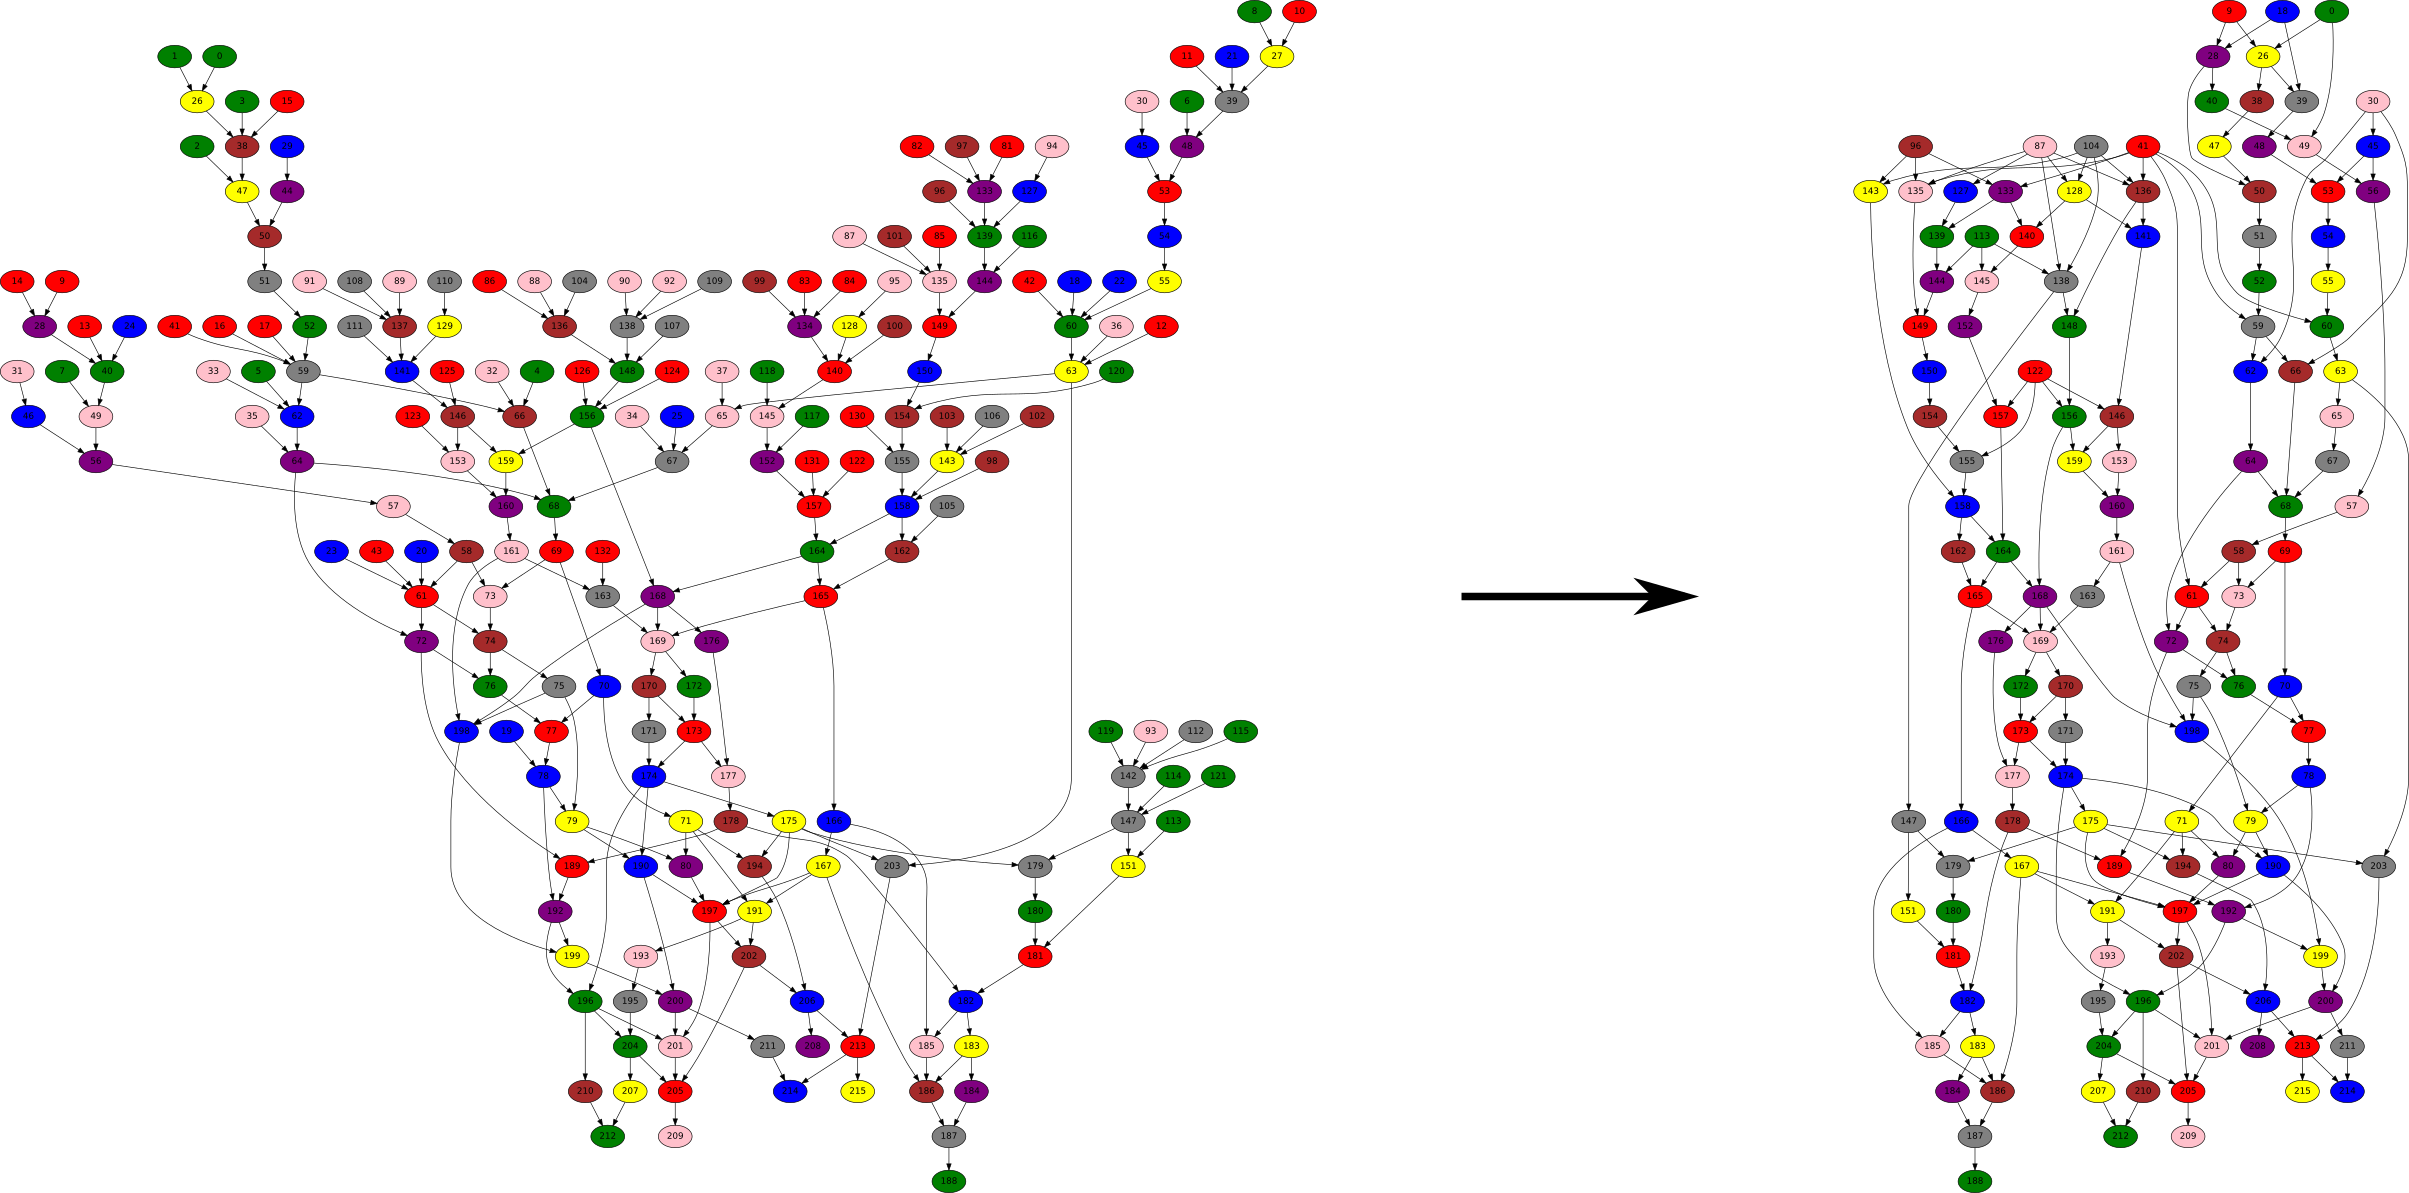
\includegraphics[width=\textwidth]{ilu_ordering2_F}
  \caption{Exemple de graphe avec un ordering nested dissection et ILU(2). Nous avons appliqué l'opérateur F.}
  \label{fig:ilu_ordering2_F}
\end{figure}


Changeons une dernière fois les paramètres du simulateur pour augmenter le grain de calcul (0,8 pour les effets caches et 0,5 pour le coût d'ordonnancement).
%
Les résultats (Table.~\ref{tab:ilu2_nested_0.8_0.5}) montrent un très léger avantage pour l'opérateur F.


%   (-_-)   %
\begin{center}
  \begin{tabular}{|c|c|c|c|c|c|c|c|c|c|c|}
    \hline
    \multicolumn{11}{|c|}{Types d'agrégations}\\
    \O & D(16) & D(64) & D(256) & D(1500) & D(2048) & F(24) & F(36) & F(42) & F(64) & C \\
    \hline
    125004 & 82073 & 78370 & 76533 & 78233 & 78180 & 77884 & 75423 & 75452 & 75555 & 117447 \\
    \hline
  \end{tabular}
  \captionof{table}{Résultats du simulateur d'exécution de tâches avec ILU(2) et une granularité grossière sur 12 coeurs de calculs.}
  \label{tab:ilu2_nested_0.8_0.5}
\end{center}


Comme nous avons pu le voir, le choix des opérateurs dépend fortement de la structure du graphe de tâche.
%
L'opérateur F sera à favoriser sur des graphes très large et peu haut.
%
Au contraire, pour des graphes très hauts et peu larges il faudra privilégier l'opérateur C.
%
L'opérateur D pourra être utilisé dans la plupart des cas même s'il ne fournit pas toujours les performances optimales.

